%%%%%%%%%%%%%%%%%%%%%%%%%%%%%%%%%%%%%%%%%%%%%%%%%%%%%%%%%%%%%%%
%
% Welcome to Overleaf --- just edit your LaTeX on the left,
% and we'll compile it for you on the right. If you give 
% someone the link to this page, they can edit at the same
% time. See the help menu above for more info. Enjoy!
%
%%%%%%%%%%%%%%%%%%%%%%%%%%%%%%%%%%%%%%%%%%%%%%%%%%%%%%%%%%%%%%%

%  My thanks to Dana Ernst of Northern Arizona University for sharing 
%    his template with me. This is largely his work.
% --------------------------------------------------------------
% This is all preamble stuff that you don't have to worry about.
% Head down to where it says "Start here"
% --------------------------------------------------------------
 
\documentclass[12pt]{article}

\usepackage[utf8]{inputenc}
\usepackage{xcolor}
\usepackage{multicol}
\usepackage{hyperref}

\usepackage[alf]{abntex2cite}

\usepackage{algorithm}
\usepackage{algpseudocode}
 
\usepackage[margin=1.5in]{geometry} 
\usepackage{amsmath,amsthm,amssymb}
\usepackage{graphicx}
\usepackage{subcaption}
\usepackage{booktabs}
\usepackage{wrapfig}
 
\newenvironment{theorem}[2][Theorem]{\begin{trivlist}
\item[\hskip \labelsep {\bfseries #1}\hskip \labelsep {\bfseries #2.}]}{\end{trivlist}}
\newenvironment{lemma}[2][Lemma]{\begin{trivlist}
\item[\hskip \labelsep {\bfseries #1}\hskip \labelsep {\bfseries #2.}]}{\end{trivlist}}
\newenvironment{conjecture}[2][Conjecture]{\begin{trivlist}
\item[\hskip \labelsep {\bfseries #1}\hskip \labelsep {\bfseries #2.}]}{\end{trivlist}}
\newenvironment{question}[2][Question]{\begin{trivlist}
\item[\hskip \labelsep {\bfseries #1}\hskip \labelsep {\bfseries #2.}]}{\end{trivlist}}
\newenvironment{corollary}[2][Corollary]{\begin{trivlist}
\item[\hskip \labelsep {\bfseries #1}\hskip \labelsep {\bfseries #2.}]}{\end{trivlist}}
\newenvironment{definition}[2][Definition]{\begin{trivlist}
\item[\hskip \labelsep {\bfseries #1}\hskip \labelsep {\bfseries #2.}]}{\end{trivlist}}

\begin{document}
 
% --------------------------------------------------------------
%                         Start here
% --------------------------------------------------------------
 
\title{Tiny Steering: Can steering survive on a fish?} % replace with an appropriate title, choose something shortish & descriptive
\author{Leonardo Valadão} % replace with your name, multiple authors go in alphabetical order by last name
\date{Aug 27, 2026}
\maketitle

{%
\centering
\textit{Instituto de Matemática e Estatística, Universidade de São Paulo} % replace the name with the name of your referee(s)
\par
}
\hrule
\vspace{.2in}

\section*{Summary}
Beaglehole et al. \cite{beaglehole2026toward} claim that the concepts ``known'' by Large Language Models are in fact linear directions in the model's activation space, that these directions can be extracted with feature-learning algorithms such as the Recursive Feature Machines (hereafter RFM), and that, once a concept has been extracted, one may \textbf{steer} the model, that is, push its outputs toward or away from that concept by purely linear computations, or \textbf{monitor} the presence of the concept by reading the model's activations. These claims are established over Llama-class models with 8 to 90 billion parameters, and it is therefore reasonable to ask whether the same results survive at much smaller scales. Do such findings endure on a model as small as $\approx 9$ million parameters? Note that a single checkpoint cannot say how the machinery scales, since that would require a ladder of model sizes and is a separate experiment altogether, but it can say whether the mechanism survives at the bottom of the range on its own merits, and a negative answer there would bound the whole claim.

This document reports a controlled replication of the aforementioned mechanisms, namely RFM extraction, additive steering, AGOP-eigenvector probing and the comparison against cheaper baselines, carried out on GuppyLM, a language model of $\approx 8.7$M parameters. We deliberately dropped the themed results of Beaglehole et al., such as steering along an anti-refusal direction to expose a model's jailbreak vulnerability, or subtracting a deception direction so that the model answers more honestly, since GuppyLM does not carry representations of such matters. Instead we ask whether linear concept extraction, additive steering and activation probing hold on language models as small as 10M parameters, restricted to the concepts the model is able to represent.

In short, the reading of concepts transfers intact, the writing of them, that is, the steering, transfers as a mechanism and yet not as a capability, and the baseline comparison is only partly testable at this scale.


\section{Fundamentals}
We begin by fixing the notation and the objects that the whole replication will use. Let
a transformer language model be composed of $L$ blocks, so that, for an input prompt $X$,
block $l$ has activations $A_l(X) \in \mathbb{R}^{t \times k }$, where $t$ is the sequence
length and $k$ the hidden dimension. As in Beaglehole et al., the feature associated with
a prompt is the last real token row of each block output, $a_l \in \mathbb{R}^k$. For each
concept we gather $n$ labelled prompts $\{X^{(i)}, y^{(i)}\}$, where $y \in \{0,1\}$
records the presence of the concept in each prompt, we run every prompt through the model,
and we stack the per-block last-token activations into the matrix
$Z_\ell \in \mathbb{R}^{n \times k}$ whose $i$-th \emph{row} is
$\left(a_\ell^{(i)}\right)^{\top}$. Note that extracting a concept vector requires no
generated text at all, only $(\text{prompt}, \text{label})$ pairs and one forward pass
each, which is what makes the data collection cheap and what the steering and monitoring
stages downstream then build on. It is on this cheapness that Beaglehole et al. rely when
they extract and steer a concept in under a minute with fewer than $500$ samples.

\subsection{Recursive Feature Machine}

The Recursive Feature Machine (RFM) of \cite{radhakrishnan2024mechanism} can be read,
informally, as a supervised and nonlinear counterpart to Principal Component Analysis
(hereafter PCA), in the sense that, where PCA returns the directions of greatest
\emph{variance} in the data, RFM returns the directions to which a fitted \emph{predictor}
is most sensitive, via the Average Gradient Outer Product (hereafter AGOP). It is not a
generalisation of PCA in the strict sense, since PCA is not a special case of the
iteration below, but the analogy is the right one for understanding what the matrix $M$ is
doing.

The predictor, for this case, is a kernel ridge regression (hereafter KRR) with a
Mahalanobis-Laplace kernel parametrized by a Positive Semidefinite (PSD) matrix $M$ with
bandwidth $\sigma$, given by

\[
  K_M(x,z) \;=\; \exp\!\left(-\frac{1}{\sigma}\sqrt{(x-z)^{\top} M (x-z)}\right)
\]

where $\sigma>0$ is the kernel bandwidth. Note that we write $\sigma$ where Beaglehole et
al. write $L$, so as to avoid a clash with the number of transformer blocks $L$.

Initialize $M_0 = I$ and, for $t = 0, \dots, T-1$:

\begin{enumerate}
  \item \textbf{Kernel ridge regression.} Fit
  \[
    \alpha_t = \left(K_{M_t}(Z,Z) + \lambda I\right)^{-1} y \;\in\; \mathbb{R}^{n},
  \]
  \[
    f_t(z) = \alpha_t^{\top} K_{M_t}(Z,z) = \sum_{i=1}^{n} \alpha_{t,i}\, K_{M_t}\!\left(a^{(i)}, z\right).
  \]

  \item \textbf{AGOP.}\footnote{We mean-centre the gradients before forming the outer product, as
pre-registered in \texttt{plans/GUPPYLM\_GUIDE.md} §1a and as implemented in
\texttt{rfm\_guppy/rfm.py}. Without centring, the top eigenvector of $M_{t+1}$ is pulled
toward the mean gradient direction rather than the direction of greatest gradient
variation.} Recompute $M$ as the average outer product of the predictor's
  input-gradients over the training points:
  \[
    M_{t+1} = \frac{1}{n}\sum_{i=1}^{n}
      \left(g^{(i)} - \bar{g}\right)\left(g^{(i)} - \bar{g}\right)^{\top},
  \]
  \[
    g^{(i)} = \nabla_z f_t\!\left(a^{(i)}\right),
    \quad \bar{g} = \frac{1}{n}\sum_{j=1}^{n} g^{(j)} .
  \]
\end{enumerate}

After $T$ iterations, the concept vector $v$ is taken as the top eigenvector of $M_T$,
with $\|v\|_2 = 1$. It is then oriented by computing the Pearson correlation $\rho$
between the projections $\{\langle a^{(i)}, v\rangle\}$ and the labels $\{y^{(i)}\}$ and
by replacing $v$ with $\operatorname{sign}(\rho)\, v$, so that a positive projection means
``more concept''. The gradient that drives the AGOP, writing
$d_i(z) = \sqrt{(z - a^{(i)})^{\top} M (z - a^{(i)})}$, is then

\[
  \nabla_z f_t(z) \;=\; -\frac{1}{\sigma}\sum_{i=1}^{n}
    \alpha_{t,i}\, K_{M_t}\!\left(a^{(i)}, z\right)\,
    \frac{1}{d_i(z)}\; M\left(z - a^{(i)}\right),
\]

with the convention that terms for which $d_i(z) = 0$ are dropped. Typical
hyperparameters are $\lambda = 10^{-3}$, $\sigma \in \{1, 10, 100\}$ and $T \leq 10$.

We prefer RFM to a plain logistic regression because the AGOP reports the directions to
which a \emph{nonlinear} predictor is sensitive, so that it can in principle surface
concept structure that a single linear separator misses. Beaglehole et al. advance that
claim under two conditions, namely abstract concepts and large models, and it is worth
keeping the conditions attached, since they decide the outcome of
§\ref{sec:baselines-anchor} below, where on the three easy and in-domain concepts
available here logistic regression matches and slightly exceeds RFM.

\subsection{Steering}

Given the concept vectors $\{v_l\}$ obtained per block, we steer during the forward pass
by adding $\varepsilon v_l$ to every token row of the output of block $l$, that is,

\[
  \tilde{A}_{\ell,i}(X) = A_{\ell,i}(X) + \varepsilon\, v_\ell
  \qquad \text{for every token position } i,
\]

where $\varepsilon$ is the control coefficient and the concept vector is taken with
$\|v_\ell\|_2 = 1$. Note that the sign of $\varepsilon$ carries the direction of the
intervention, since a positive $\varepsilon$ steers towards the concept and a negative one
steers away from it. If one wishes to steer a group of concepts simultaneously, one shall
use a combination of the corresponding vectors.

\subsection{Monitoring}

For monitoring rather than steering, we keep the top $p$ eigenvectors $\{v_{l,j}\}$ per
block instead of a single one. The feature for prompt $i$ is then the set of projections
$\langle a_l^{(i)}, v_{l,j} \rangle$ over all blocks $l$ and all components $j$, which is
a vector in $\mathbb{R}^{Lp}$. On these features we train a classifier under one of two
strategies, either per-block, training one classifier per block and keeping the best of
them, or aggregate, concatenating all blocks and training a single classifier. The
evaluation is made by AUROC (Area Under the Receiver Operating Characteristic curve).

\subsection{Baselines}

RFM is compared against three cheaper extraction methods, described below. All three
operate on the mean-centred training activations, return a unit vector, and are oriented
by the same Pearson-sign rule as RFM, so that the comparison between them is a comparison
of directions and of nothing else.

\begin{itemize}
  \item \textbf{PCA.} Pair the $j$-th positive sample with the $j$-th negative sample,
  $j = 1, \dots, m$ with $m = \min(n_+, n_-)$, and form the difference matrix $D$ with
  rows $D_j = a^{(\pi^+(j))} - a^{(\pi^-(j))}$. Mean-centre it, $\tilde{D} = D - \bar{D}$,
  so that $v$ is the top right singular vector of $\tilde{D}$, equivalently the top
  eigenvector of $\tilde{D}^{\top}\tilde{D}$.

  \item \textbf{Difference-in-means.}
  $v = \dfrac{\mu_1 - \mu_0}{\left\|\mu_1 - \mu_0\right\|_2}$, where
  $\mu_c = \operatorname{mean}(S_c)$ is the mean activation of class $c$.

  \item \textbf{Logistic regression.} $v = w / \|w\|_2$, for the fitted coefficient
  vector $w$, with the inverse-regularisation strength $C$ swept on the validation split.
\end{itemize}


\section{GuppyLM}
GuppyLM is a deliberately tiny, open-source and character-driven language model, themed as
a fish. It was built for teaching, being a complete and readable reference implementation
of a small instruction-tuned transformer, and it is a good mechanism testbed precisely
because it is small enough to be fully controllable and inspectable while still being a
real instruction-tuned transformer. Its architecture and training data are summarised in
Table~\ref{tab:guppylm_properties}.

\begin{table}[htbp]
\centering
\caption{GuppyLM architecture and training data.}
\label{tab:guppylm_properties}
\begin{tabular}{l l}
\toprule
\textbf{Property} & \textbf{Value} \\
\midrule
Parameters &  $\approx 8.73$M \\
Transformer blocks & 6 \\
Hidden dimension $k$ & 384 \\
Vocabulary capacity & 4096 \\
Training data & \href{https://huggingface.co/datasets/arman-bd/guppylm-60k-generic}{$\approx 60$k rows over 60 categories} \\
\bottomrule
\end{tabular}
\end{table}

Each block outputs a residual-stream tensor of shape $[B, T, 384]$, which matches the
method of Beaglehole et al. for reading from and writing to the model. The model is
trained on 60 templated conversational categories, such as food, weather, greetings and
moods, and those categories are the only concepts GuppyLM can plausibly be expected to
represent, given that they are the whole of its training distribution, so we restrict this
work to them. Note that whether the model also carries structure outside these categories
is not something we tested, and it is not something a probe restricted to these labels
could see.

One convenient consequence of GuppyLM's small scale is that its per-block activation norms
are small and can simply be measured. The median $\|a_\ell\|_2$ over the cached training
activations runs $11.9,\ 22.8,\ 27.6,\ 30.7,\ 30.9,\ 29.7$ from block 0 to block 5, a
roughly $2.6$-fold rise that peaks at block 4, as shown in
Figure~\ref{fig:activation_norms}. Consequently a fixed absolute perturbation is a nudge
at block 5 and a wrecking ball at block 0, which is exactly why the absolute steering
coefficients of Beaglehole et al. cannot be copied over.

\begin{figure}[htbp]
    \centering
    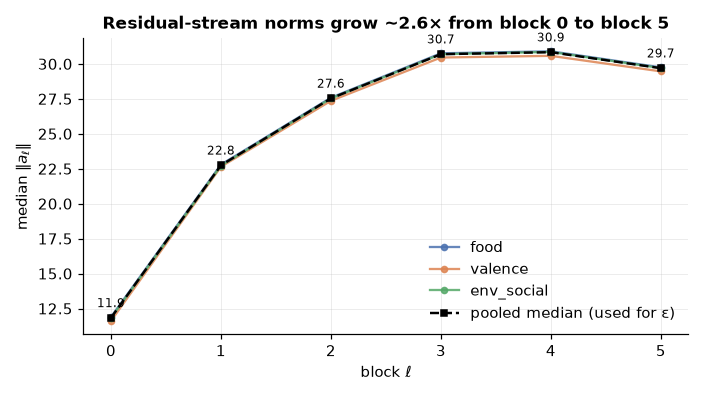
\includegraphics[width=0.75\textwidth]{imgs/01_activation_norms.png}
    \caption{The three concepts agree almost exactly, and the median (dashed) is a safe scale to normalise by.}
    \label{fig:activation_norms}
\end{figure}

It is possible to see in the figure that the three concepts agree almost exactly on the
per-block norm profile, which means the median is a safe common scale to normalise by, and
it is that median which defines the relative coefficient $r$ used throughout the steering
experiments below.


\section{Steering on a tiny model}
The aim of this section is to describe the replication itself, from the activation harness
up to the comparison against the cheaper extraction baselines. For each of the 6 blocks of
the model we register forward hooks, capture each block's output $[B, T, 384]$, and
extract the last non-pad token row per prompt, which yields
$A \in \mathbb{R}^{n \times 6 \times384}$. The harness was checked for determinism, with
\verb|model.eval()|, and for padding invariance, that is, a prompt's activation is
independent of the right-padding length, a property which we verified to the order of
$7\times 10^{-7}$.

\subsection{Concept datasets}

Because the raw user inputs are heavily templated, with only about 4 to 34 unique strings
per category, we use the full ChatML exchange, that is, the user turn together with
GuppyLM's response, as the prompt, which yields hundreds of distinct texts per category.
On those we build three binary concepts, each of them defined as a contrast between groups
of categories, as reported in Table~\ref{tab:concept_categories}.


\begin{table}[htbp]
\centering
\caption{The three binary concepts, defined as category contrasts.}
\label{tab:concept_categories}
\begin{tabular}{@{}l p{4.2cm} p{4.6cm} c@{}}
\toprule
\textbf{Concept}& \textbf{Positive Categories} & \textbf{Negative Categories} & \textbf{N/class} \\
\midrule
food &  food, taste & weather, seasons, tv, music, glass, rain, outside & 300 \\
valence &  happy, excited, love, curious & scared, fear, bored, tired & 100 \\
env\_social &  water, filter, temp\_hot, temp\_cold, algae & greeting, bye, friends, visitors, lonely & 300 \\
\bottomrule
\end{tabular}
\end{table}

Each concept is class-balanced and split 60/20/20 into train, validation and test sets
over \emph{unique} exchange strings, with the absence of prompt leakage across splits
asserted at build time. That gives 360/120/120 examples for \verb|food| and
\verb|env_social|, and 120/40/40 for \verb|valence|. Note that \verb|valence| is therefore
the smallest of the three concepts by a factor of three, which is a fact worth keeping in
mind when reading its results below, since every difference reported for that concept
rests on a proportionally smaller sample.

\subsection{RFM implementation}

The RFM was implemented as a Python package, \verb|rfm_guppy|. The functions of its core,
namely \verb|laplace_kernel|, \verb|rfm_fit|, \verb|agop_grad|, \verb|top_eigvectors|,
\verb|orient| and \verb|extract_concept_vector|, perform the concept-vector extraction
using mean-centred inputs, vectorised AGOP gradients with the $d_i = 0$ guard, \verb|eigh|
on the $384 \times 384$ PSD matrix, and hyperparameter selection by maximising the
validation $|\rho|$, that is, the absolute Pearson correlation between
$\langle a, v \rangle$ and $y$, over $\sigma \in \{1, 10, 100\}$, $T \in \{1, \dots, 10\}$
and $\mathrm{normalize} \in \{\mathrm{False}, \mathrm{True}\}$.

Writing the gradient of every training point at once as an $[n, n, k]$ tensor would cost
roughly 400\,MB, so we rewrite it as a pair of matrix products. Define

\[
  W_{ij} = \frac{\alpha_j \, K_M\!\left(a^{(i)}, a^{(j)}\right)}
                {\sigma \, d_j\!\left(a^{(i)}\right)},
  \qquad
  W_{ij} = 0 \ \text{ when } d_j\!\left(a^{(i)}\right) = 0,
\]

so that the stacked gradient matrix $G \in \mathbb{R}^{n \times k}$, whose $i$-th row is
$\nabla_z f_t(a^{(i)})^{\top}$, is given by

\[
  G = -\left(\operatorname{diag}\!\left(W \mathbf{1}\right) Z_c \;-\; W Z_c\right) M ,
\]

with $\mathbf{1} \in \mathbb{R}^{n}$ the all-ones vector and $Z_c$ the mean-centred
activations. Peak memory is then $O(nk + n^2)$ rather than $O(n^2 k)$. The $T$ sweep also
runs incrementally, in the sense that iteration $T+1$ continues from the matrix $M$
obtained at iteration $T$.

Before running on real data, we gate the implementation on a synthetic recovery test. We
generate $n = 1000$ standard-normal points $z_i \in \mathbb{R}^{k}$ with $k = 384$ and
label them by $y_i = \langle z_i, u \rangle$ for a hidden direction $u$ with
$\|u\|_2 = 1$, and we then confirm that the top eigenvector $v$ returned by RFM aligns
with $u$. The pre-declared acceptance criterion is $|\cos(v, u)| > 0.90$, and the run
achieves $|\cos(v, u)| = 0.9528$.

Two details of the gate are deliberate. Firstly, the 1{,}000 points are split 800/200 into
train and validation, so that the reported $|\cos(v,u)|$ is obtained from the
hyperparameters that maximise the validation $|\rho|$, exactly as on the real concepts.
Secondly, the labels are real-valued here rather than the $y \in \{0,1\}$ of §2, since
recovering a direction in $\mathbb{R}^{384}$ from 800 points is a question about the AGOP
machinery, and thresholding $\langle z, u \rangle$ to a sign would discard most of the
information about $u$ unless $n \gg k$. Note that the gate is therefore an easier problem
than the concepts that follow, by construction, which means it is a correctness check on
the implementation and not a difficulty benchmark. The behaviour of the recursion on this
gate is shown in Figure~\ref{fig:agop_convergence}.

\begin{figure}[htbp]
    \centering
    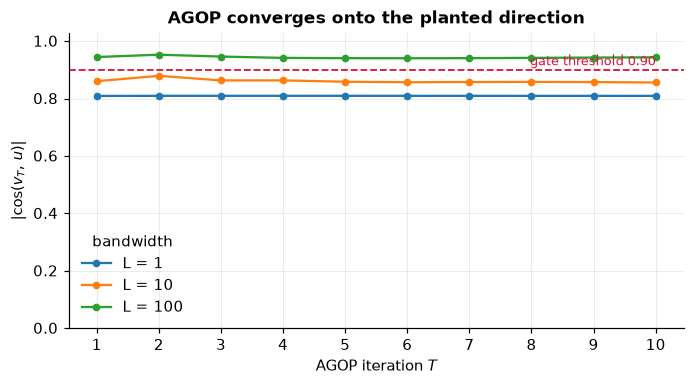
\includegraphics[width=0.75\textwidth]{imgs/02_agop_convergence.png}
    \caption{Unrolling the AGOP loop by hand shows the convergence curve is flat.}
    \label{fig:agop_convergence}
\end{figure}

What is flat here is the \emph{recursion}, and not the AGOP. Since $T$ counts the steps
taken from $M_0 = I$, the vector at $T = 1$ is already a full AGOP, one formed from the
gradients of a predictor fitted with the ordinary Laplace kernel, and because $y$ is
exactly linear in $\langle z, u \rangle$ that single step is enough. It is possible to see
that $\sigma = 100$ reaches $|\cos(v,u)| = 0.945$ at $T = 1$ and that the following nine
iterations change nothing, while $\sigma = 1$ sits at $0.809$ and $\sigma = 10$ at $0.860$
and neither of them climbs out. What the sweep buys on this gate is therefore the
\emph{bandwidth} and not the iteration count, which is exactly why $\sigma$ is swept here
rather than copied from Beaglehole et al. The iteration earns its keep on real
activations, where it drives $M$ toward rank 1\footnote{Rank(M) = the number of nonzero eigenvalues for that matrix. When M is rank 1, one eigenvalues is nonzero and all others are zero, which is equivalent to saying $M$ factors as a single outer product $M = \lambda_1 v_1 v_1^{\top}$ with $\|v_1\|_2 = 1$}, which is a different matter from finding the direction in the first place.

\subsection{Concept-vector extraction}

Running RFM for the concept extraction, we obtain a strong linear separability for every
concept and at every block except the earliest one, as reported in
Table~\ref{tab:rfm-val-pearson}.

\begin{table}[htbp]
\centering
\caption{Validation $|\text{Pearson}|$ (RFM), per block}
\label{tab:rfm-val-pearson}
\begin{tabular}{c c c c}
\toprule
\textbf{Block} & \textbf{food} & \textbf{valence} & \textbf{env\_social} \\
\midrule
0 & 0.906 & 0.507 & 0.735 \\
1 & 0.973 & 0.899 & 0.941 \\
2 & 0.975 & 0.908 & \textbf{0.950} \\
3 & \textbf{0.978} & 0.905 & 0.944 \\
4 & 0.977 & \textbf{0.918} & 0.942 \\
5 & 0.977 & 0.908 & 0.943 \\
\bottomrule
\end{tabular}
\end{table}

Note that block 0 is consistently weaker for every concept, which suggests that one block
of attention and MLP is not enough to build the feature, whereas blocks 1--5 all give a
projection strongly correlated with the label. The concepts \verb|food| and
\verb|env_social| are topic distinctions, exactly the kind of thing a small model encodes
bluntly, while \verb|valence| is the weak one throughout, and that is itself a finding,
since the mechanism does not report the same success on every concept it is handed, which
is what one wants from a measurement rather than from a demonstration.

\begin{figure}[htbp]
    \centering
    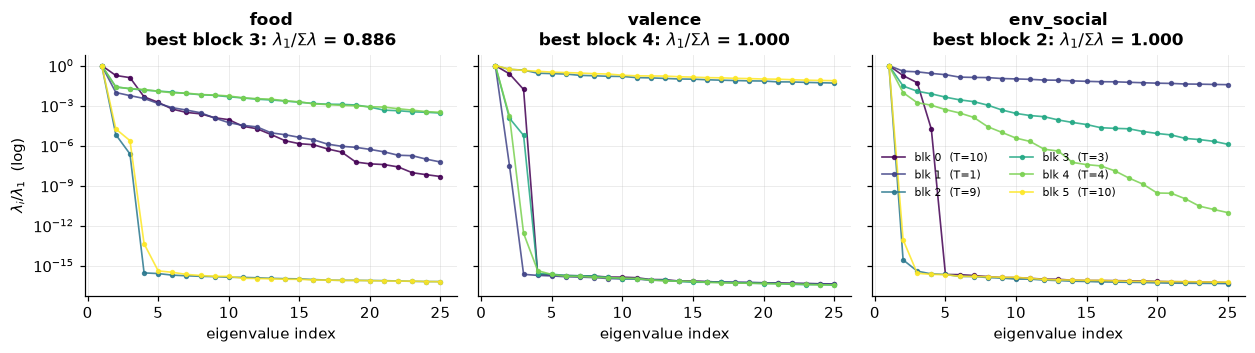
\includegraphics[width=0.75\textwidth]{imgs/03_agop_spectra.png}
    \caption{How rank-1 are the concepts?}
    \label{fig:agop_spectra}
\end{figure}

We also turn to study how rank-1 the concepts are, using two distinct quantities. The
curve in Figure~\ref{fig:agop_spectra} is the normalised spectrum $\lambda_j / \lambda_1$
against the eigenvalue index $j$, while the summary statistic quoted below is
$\lambda_1 / \sum_j \lambda_j$, the fraction of the spectral mass carried by the top
direction. Each block is plotted at whatever iteration $T$ the validation sweep selected
for it, and the spectrum depends strongly on that $T$. Where the sweep chose many
iterations the collapse is virtually total, as with \verb|env_social| block 2, selected at
$T = 9$, which has $\lambda_2 / \lambda_1 \approx 3 \times 10^{-15}$, that is, numerically
rank 1. Where it chose $T = 1$ the matrix has barely been re-weighted and the spectrum is
still broad, as with \verb|valence| block 5, which sits at
$\lambda_1 / \sum_j \lambda_j = 0.147$. At the block where the validation $|\rho|$ is
highest for each concept, $\lambda_1 / \sum_j \lambda_j$ is $0.886$ (\verb|food|, block
3), $1.000$ (\verb|valence|, block 4) and $1.000$ (\verb|env_social|, block 2), so that
there the concept really is a single direction. Note that this block is reported for
description only, since steering perturbs all six blocks at once, each with its own
$v_\ell$, and the monitoring probe reads all six, so that nothing downstream selects on
it.

The more interesting observation is that the two properties come apart. The concept
\verb|valence| at block 2 has a thoroughly non-degenerate $M$, with
${\lambda_1}/{\sum \lambda} = 0.186$, and still reaches a validation $|\rho| = 0.908$,
essentially matching the rank-1 solution of block 4 at $0.918$. We conclude, therefore,
that the concentration of the AGOP spectrum is not a prerequisite for the top eigenvector
being a good concept direction, for the direction is recoverable well before $M$ has
finished collapsing onto it.

\subsection{Steering}

We now turn to the steering itself, and the most interesting lesson we found is that
whoever wishes to steer should not blindly reuse the coefficients of Beaglehole et al.
The values $\varepsilon \in \{0.1, ..., 0.65\}$ reported there are tuned to Llama's
activation scale, while GuppyLM's activation norms are 12-31, so that such small
$\varepsilon$'s would do very little. Instead we choose

\[
  \varepsilon_\ell = r \cdot \operatorname*{median}_{i} \left\| a_\ell^{(i)} \right\|_2 ,
\]

the median being taken over all cached training activations, pooled across the three
concepts. Since $\|v_\ell\|_2 = 1$, the relative coefficient $r$ is exactly the size of
the perturbation as a fraction of the typical residual-stream norm at that block, and it
is $r$, and not $\varepsilon$, that ports across models. We sweep
$r \in \{-4, -2, -1, -0.5, -0.25, 0, +0.25, +0.5, +1, +2, +4, +8 \}$. Note that the trick
here is the hook, for returning a tensor from a PyTorch forward hook replaces the module
output, and the hook fires on every generated token. Table~\ref{tab:steering_samples}
shows sample generations for the probe prompt ``How are you doing today?''.

\begin{table}[htbp]
\centering
\caption{Sample generations to the probe prompt \textit{``How are you doing today?''} under steering at $r=0$ (baseline) versus $r=+0.25$.}
\label{tab:steering_samples}
\small
\begin{tabular}{@{}l p{5.5cm} p{5.5cm}@{}}
\toprule
\textbf{Concept} & \textbf{$r = 0$ (baseline)} & \textbf{$r = +0.25$} \\
\midrule
food &
\textit{``i'm a little fish. i am small but i have opinions. mostly about food.''} &
\textit{``whole palate palate palate promise to promise to best excited palate best \ldots''} \\
\addlinespace
valence &
(same baseline) &
\textit{``tv means floating someone wanting chestpick now either excited. noticed bit happ\ldots''} \\
\addlinespace
env\_social &
(same baseline) &
\textit{``if can breathe can if breathe can if if i breathe breathe more breathe if if if\ldots''} \\
\bottomrule
\end{tabular}
\end{table}

The intervention unmistakably works, and it is unmistakably blunt. A direction fitted to
$(\text{prompt}, \text{label})$ pairs, which never saw a single generation, drags the
output onto tank-and-water vocabulary from a probe prompt that mentions no such thing, so
that the causal claim replicates. However, if one reads the text rather than the keywords,
what is there is repetitive and barely grammatical vocabulary drift, and not a fluent fish
talking about its tank. Two things plausibly contribute, and we can separate neither of
them with a single model. The perturbation may simply be larger than an 8.7M-parameter
residual stream has slack to absorb, and the vectors are fitted on the last-token
activation of a \emph{complete} ChatML exchange while steering writes them into every
position of a \emph{partial} one, so that the direction is being applied to a state
distribution on which it was never estimated.

We scored the steers over a set of 7 neutral probe prompts, 12 values of $r$ and 3
concepts by lexicon hit rate, and the three concepts tell rather different stories, as can
be seen in Figure~\ref{fig:steering_lexicon_sweep}.

\begin{figure}[htbp]
    \centering
    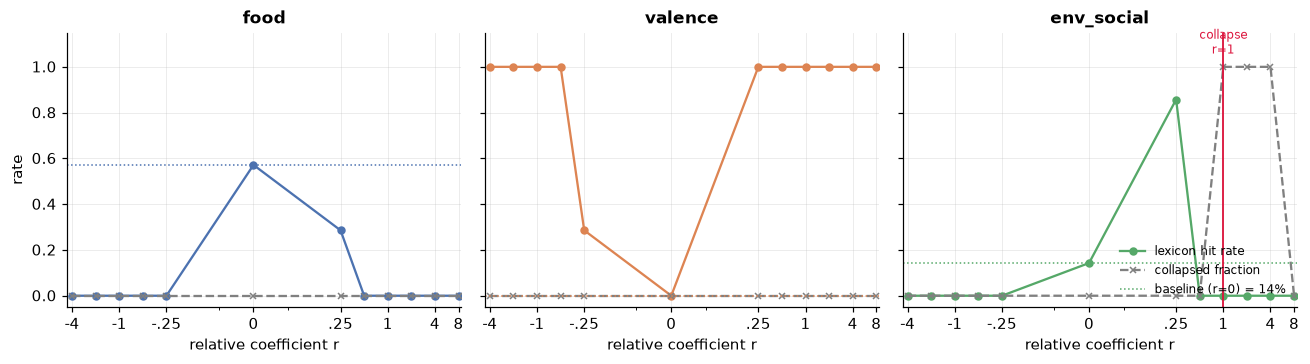
\includegraphics[width=0.75\textwidth]{imgs/04_steering_lexicon_sweep.png}
    \caption{Three shapes, three different failures of the metric.}
    \label{fig:steering_lexicon_sweep}
\end{figure}

The concept \verb|env_social| behaves as Beaglehole et al. would predict, going from a
baseline of 14\% to 86\% at $r = +0.25$ and then collapsing, with 7 of 7 generations
degenerate at $r = +1, +2, +4$. That is a narrow usable band with a hard ceiling, exactly
the described shape, though a thin one, since the 14\% baseline is a single generation
containing \emph{hello}, a word taken from the concept's \emph{negative} categories, and
the 86\% is a single keyword, \emph{cold}, appearing in 6 generations out of 7. Note that
no other positive-pole word fires anywhere in the sweep.

The concept \verb|food| fails by this measure, and it fails instructively. Its baseline at
$r = 0$ is already 57\%, because a fish whose entire personality is thinking about food
mentions food unprompted, and steering cannot add a concept that is already saturated, so
that it can only break the sentences that carried it and the hit rate consequently goes
\emph{down}, from 57\% to 29\% at $r = +0.25$ and then to 0\% everywhere else. The drop is
mostly not even a matter of fluency, since the word that dominates the generations at
$r = +0.25$ is \emph{palate}, with 56 occurrences across the seven outputs, which is
squarely on-concept and simply absent from the thirteen-word lexicon. What this curve
measures, therefore, is the keyword list missing the vocabulary that the steering
produced.

The concept \verb|valence| reports 100\% at $r = \pm 0.5$ and beyond, in both directions.
That is not symmetric steering, it is the scalar metric discarding a sign that it did in
fact record. The \verb|valence| lexicon spans both poles, with \emph{happy, excited, joy}
alongside \emph{scared, fear, tense, stiff, hide}, so that a push either way scores a hit,
and yet the words themselves separate cleanly, since every negative $r \leq -0.5$ fires
\emph{hide} in 7 generations out of 7 and every positive $r \geq +0.25$ fires
\emph{excited} in 7 out of 7, with no crossover. The hit \emph{rate} is sign-blind, the
hits are not. It is worth stating this plainly, because it is bidirectional evidence that
does not come from the probe, and so is not subject to the circularity discussed below.
The same two-poled construction applies to \verb|env_social|, whose lexicon also contains
its negative categories (\emph{hello, hi, friend, bye}).

One caveat is easy to miss, and it matters for reading every ``collapsed'' figure quoted
above. The detector flags a generation only when a single word takes more than 60\% of the
output, so that the \verb|food| generations at $r = +0.25$ sit between 0.28 and 0.41 by
that measure and are flagged clean while reading as
\emph{``whole palate palate palate promise to promise to best\ldots''}, and
\verb|env_social| at $r = +8$ scores 0.59 and is flagged clean while producing the same
degenerate \emph{``if can breathe can if\ldots''} string that scores 0.61 and is flagged
collapsed at $r = +4$. Note that a zero in the collapsed column means the text is not
maximally repetitive, but it does not mean the text is coherent.

The honest result for this steering phase is that the direction is real and causal, and
yet at every $r \neq 0$ we tested the fluency degrades. It appears that an
8.7M-parameter model has too little slack to absorb a perturbation large enough to matter
without losing the thread of a sentence.

For the steering evaluation, since we have no GPT-4o judge available at this scale, the
second metric is a probe score, obtained by feeding the generated text back through the
model as a full ChatML exchange and reading the concept probability reported by the
monitoring probe. A generation counts as steered if the probe score is greater than 0.5 or
if it hits the lexicon, and the resulting success rates are reported in
Table~\ref{tab:steering_success}.

\begin{table}[htbp]
\centering
\caption{Steering-success rate (probe score $>0.5$ or lexicon hit) at $r=0$ versus the best positive-$r$ coefficient in the sweep, per concept.}
\label{tab:steering_success}
\begin{tabular}{@{}lccc@{}}
\toprule
\textbf{Concept} & \textbf{Baseline} & \textbf{Best} & \textbf{Best $r$} \\
\midrule
food        & 71.4\% & 100.0\% & $+0.25$ \\
valence     & 71.4\% & 100.0\% & $+0.25$ \\
env\_social & 28.6\% & 100.0\% & $+0.25$ \\
\bottomrule
\end{tabular}
\end{table}

\begin{figure}[htbp]
    \centering
    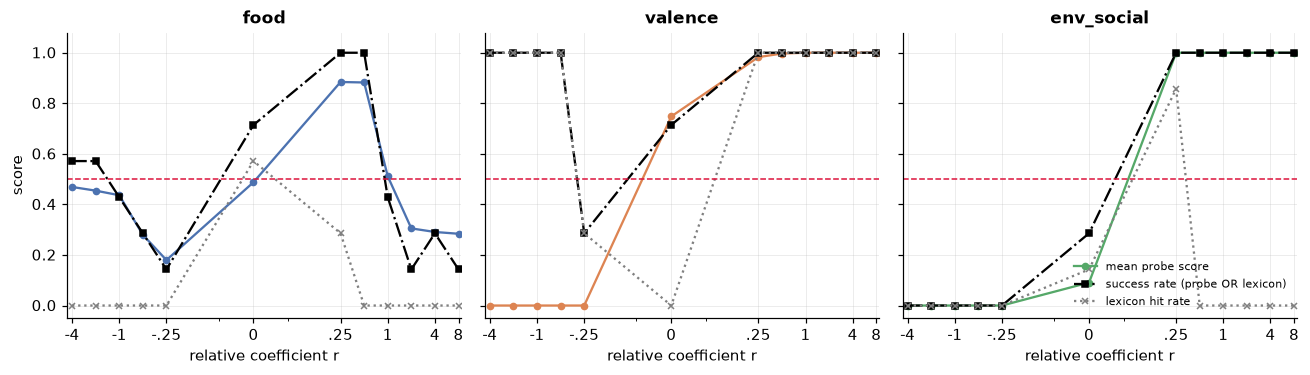
\includegraphics[width=0.75\textwidth]{imgs/05_steering_probe_sweep.png}
    \caption{The probe (solid) and the lexicon (dotted) disagree everywhere it matters.}
    \label{fig:steering_probe_sweep}
\end{figure}

The activations did move, and it was we who moved them by steering, so that this metric is
partially circular, given that the probe reads the top AGOP eigenvectors and the steering
vector is itself the top AGOP eigenvector. In fairness to the probe, it is not merely
reacting to being perturbed, since it tracks the sign of $r$ on every concept
(\verb|valence| and \verb|env_social| fall to exactly 0.00 under negative steering and sit
at 1.00 under positive steering, and even \verb|food| separates 0.18 to 0.47 under
negative steering from 0.88 at $r = +0.25$), which is genuine bidirectional information.
What the probe cannot notice is that the sentence carrying that direction stopped being a
sentence. The 100\% figure is therefore not independent evidence that steering works, and
it should not be read as such.

\subsection{Monitoring}

Using the top $p=3$ AGOP eigenvectors per block, each prompt becomes a projection vector
in $\mathbb{R}^{18}$, that is, $6$ blocks times $3$ components, which is a 128-fold
compression of the raw $6 \times 384$ activations. A logistic-regression probe, with a
standardizer in front and $C$ swept on validation, is trained under both the
per-block-best and the aggregate strategies and evaluated on the held-out test split. For
all three concepts the test AUROC is $1.000$. The per-block strategy reports block 1 as
the best one for each of them, but that is a tie-break and not a result, since on
validation blocks 1--5 all score exactly $1.000$ and only block 0 is weaker ($0.998$ for
\verb|food|, $0.913$ for \verb|valence| and $0.939$ for \verb|env_social|), so that block
1 is merely the first index of a five-way tie.

The separation is visible before any classifier is fitted, as one can see by projecting
the test split onto the first two AGOP eigenvectors of each concept's best block, which is
what Figure~\ref{fig:agop_projection_scatter} displays.

\begin{figure}[htbp]
    \centering
    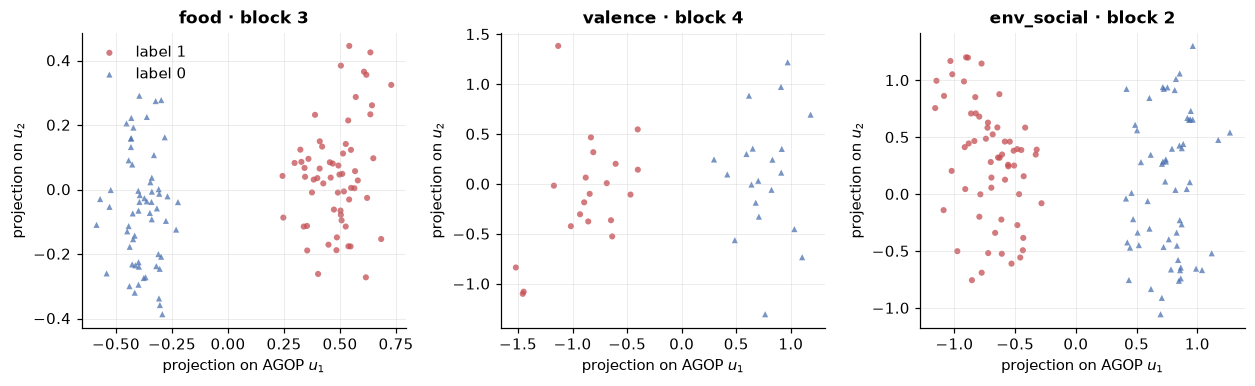
\includegraphics[width=0.75\textwidth]{imgs/06_agop_projection_scatter.png}
    \caption{Two clouds, split by the horizontal axis alone.}
    \label{fig:agop_projection_scatter}
\end{figure}

The test AUROC equals 1.0 across the board for both strategies, and every ROC curve is a
right angle. Even a single feature suffices, since the first AGOP eigenvector alone
reaches an AUROC of 1.0 unaided on all three concepts. The second and third eigenvectors
are much weaker, with $u_2$ scoring $0.679$, $0.617$ and $0.599$ and $u_3$ scoring
$0.519$, $0.645$ and $0.705$ on \verb|food|, \verb|valence| and \verb|env_social|
respectively. Note that four of those six values are far enough above $0.5$ to say that
the trailing directions carry some residual class signal, which is a small qualification
of the strict rank-1 picture, while the $u_3$ of \verb|food| at $0.519$, on a 120-example
test split, is indistinguishable from chance.

A ceiling is not the same thing as a strong result, and three properties of this setup
make it an easy one. The concepts are the model's \emph{own} training categories rather
than emergent properties, the test splits are small (120, 40 and 120 examples), and the
positive and negative classes are drawn from disjoint and plainly distinct groups of
categories. A fourth property is specific to the way the data were built, for since a
prompt is a complete exchange containing GuppyLM's own answer, the probe is reading the
last-token state of a text that already states its topic lexically, so that some of what
it certifies is topic classification rather than the recovery of a latent concept. A
perfect score says that the linear read-out mechanism is intact at 8.7M parameters, but it
says nothing about how the method behaves on a genuinely hard concept, because none was
presented.

\subsection{Baselines}
\label{sec:baselines-anchor}

We ran PCA, difference-in-means, logistic regression and RFM through the same pipeline,
that is, the same splits, the same probe, the same success threshold, and a steering sweep
over $r \in \{0, \pm 0.25, \pm 0.5, \pm 1, \pm 2\}$, which is narrower at the extremes
than the twelve-point sweep used above, though every method's best positive coefficient
falls at $r = +0.25$ and therefore well inside it. The quality of the directions obtained
by each method is reported in Table~\ref{tab:baselines_val_rho}.

\begin{table}[htbp]
\centering
\caption{Direction quality, validation $|\rho|$ (Pearson correlation with the label) at each method's best block.}
\label{tab:baselines_val_rho}
\begin{tabular}{@{}lccc@{}}
\toprule
\textbf{Method} & \textbf{food} & \textbf{valence} & \textbf{env\_social} \\
\midrule
PCA        & 0.929 & 0.154 & 0.490 \\
DiffMeans  & 0.975 & 0.800 & 0.914 \\
LogReg     & \textbf{0.986} & \textbf{0.960} & \textbf{0.972} \\
RFM        & 0.978 & 0.918 & 0.950 \\
\bottomrule
\end{tabular}
\end{table}

The separation predicted by Beaglehole et al. does appear, but only against PCA, and only
on the two harder concepts, since PCA collapses to 0.15 on \verb|valence| against RFM's
0.92 and manages 0.49 on \verb|env_social| against 0.95. The reason is structural, for PCA
takes the top direction of variance in the difference matrix, and variance is not the
class boundary, so that when two classes differ subtly but each of them has plenty of
internal spread, the top principal component tracks the spread. The supervised methods
stay much closer to one another, and note that logistic regression actually edges RFM out
on all three concepts by this measure. The monitoring performance of each method is
reported in Table~\ref{tab:baselines_auroc}.


\begin{table}[htbp]
  \centering
  \caption{Monitoring AUROC (test split, aggregate probe) across extraction methods.}
  \label{tab:baselines_auroc}
  \small
  \begin{tabular}{@{}lccccc@{}}
    \toprule
    \textbf{Concept} & \shortstack{\textbf{RFM}\\3 eigvecs (18 feat)} & \shortstack{\textbf{RFM}\\top eigvec (6 feat)} & \shortstack{\textbf{DiffMeans}\\(6 feat)} & \shortstack{\textbf{LogReg}\\(6 feat)} & \shortstack{\textbf{PCA}\\(6 feat)} \\
    \midrule
    food        & 1.0000 & 1.0000 & 1.0000 & 1.0000 & 0.9947 \\
    valence     & 1.0000 & 1.0000 & 1.0000 & 1.0000 & 0.7425 \\
    env\_social & 1.0000 & 1.0000 & 1.0000 & 1.0000 & 0.8992 \\
    \bottomrule
  \end{tabular}
\end{table}

Every method here gets the same budget of 6 features per block, one direction each, with
the exception of the first RFM column, which is kept at its native 3-eigenvector and
18-feature setup as a control. The three supervised methods, namely RFM, DiffMeans and
LogReg, sit on the AUROC ceiling in every configuration, with only PCA separating from the
pack (0.74 on \verb|valence| and 0.90 on \verb|env_social|). Note that, stripped to one
direction per block, RFM still scores 1.000, so that the extra eigenvectors were never
carrying the result, and yet trimming them away does not open any daylight against
DiffMeans or LogReg either.

The steering comparison, in contrast, does not rank the methods at all. The committed
Phase-8 table reports 100\% steering success for all four methods, which reads like a
four-way tie but is in fact a broken measurement, since under negative steering on
\verb|food| PCA scores 1.000 at $r = -2$, and DiffMeans at 0.841 and LogReg at 0.889 also
clear the 0.5 threshold, so that those methods are credited with ``success'' for steering
in the wrong direction. Two separate defects produce that outcome, and both of them belong
to the metric rather than to the methods. The first is that the probe is built from the
RFM eigenbasis and is scored on the \emph{regenerated} text, so that it need not respond
antisymmetrically to a perturbation along someone else's direction, and indeed on
\verb|food| it saturates at both signs for PCA and DiffMeans while on \verb|env_social| it
reads every baseline's negative sweep correctly at $0.000$. The second is the disjunction
in the criterion itself, since success is defined as ``probe $>0.5$ \emph{or} lexicon
hit'', so that LogReg on \verb|valence| records 100\% success at $r = -2, -1, -0.5$ on
lexicon hits alone, with a probe score of exactly $0.000$. Only the RFM row is measured by
a stick that is aligned with it, at $0.454$ for $r = -2$ and $0.436$ for $r = -1$ on
\verb|food|.

In summary, the baseline comparison shows exactly two things cleanly, namely that RFM
beats PCA (validation $|\rho|$ of 0.92 against 0.15 on \verb|valence| and 0.95 against
0.49 on \verb|env_social|, and monitoring AUROC of 1.000 against 0.74 and 1.000 against
0.90), and that RFM, DiffMeans and LogReg are indistinguishable, tied at the AUROC ceiling
with LogReg even edging RFM out on validation $|\rho|$, while the steering-based
comparison, being sign-blind for the three baselines, adds nothing to either finding. This
is not a failure to replicate, and it is what the reasoning of Beaglehole et al. itself
predicts, since RFM's advantage is supposed to appear where the class boundary is neither
the direction of greatest variance nor a simple mean shift, and three in-domain
topic-and-mood distinctions in an 8.7M-parameter fish chatbot are not that test, and were
never going to be.

\subsection{Main Findings}

If we line up what Beaglehole et al. claim against what actually happened at 8.73M
parameters, the result splits cleanly into three groups, namely the claims that hold
outright, the claims that hold in a narrower sense than stated, and one claim that never
gets a fair test at all. We shall discuss each of the three in turn.

Extraction and monitoring hold outright. Linear concept extraction via AGOP works, since
the planted-direction gate recovers the hidden vector at $|\cos| = 0.953$ and, on real
concepts, labels alone drive the validation $|\rho|$ as high as 0.978. The probe AUROC on
held-out data is a perfect 1.000 for all three concepts, far above the ``$\gg 0.5$'' bar
of Beaglehole et al., though this is a ceiling and is reported as one, and not as proof
that the method is hard to beat. RFM also beats PCA on monitoring exactly as predicted,
1.000 against an overall 0.879.

The claim that concepts are near rank-1 is true, but only with a qualifier that Beaglehole
et al. do not need to state. At each concept's best block, $\lambda_1/\sum\lambda$ is
0.886, 1.000 and 1.000, which is genuinely single-direction. That number, however, depends
on the hyperparameters that the validation sweep happened to select, since every block
whose spectrum stayed broad was selected at $(\sigma = 100, T = 1)$ and every collapsed
one at $\sigma \in \{1, 10\}$ with a larger $T$, so that bandwidth and iteration count move
together and this sweep cannot attribute the collapse to either of them alone. What the
data do show is the direction that matters, namely that a block stopped at $T = 1$, with a
spectrum nowhere near collapsed, still yields a good concept vector, so that rank-1-ness
is not a precondition for the top eigenvector being useful. Isolating what causes the
collapse would require a sweep over $T$ at fixed $\sigma$, which we did not run.

Steering is where the single claim of Beaglehole et al. turns out to be two claims, and
only one of them survives. Does the direction causally move the model? It does,
unambiguously, since the output vocabulary drags hard toward the concept and the effect
carries the sign of the perturbation rather than merely its size, in the sense that the
probe score tracks $\operatorname{sign}(r)$ on all three concepts and, on \verb|valence|,
the generated words do so as well (\emph{hide} under every negative $r$ and
\emph{excited} under every positive one), which the aggregate hit rate hides because the
word list spans both poles. The small-coefficient-works and large-coefficient-collapses
pattern also shows up (\verb|env_social| is flagged degenerate 7 for 7 at
$r = +1, +2, +4$), with the caveat recorded above that the flag itself stops firing at
$r = +8$ on text that has not recovered. Does the steering produce coherent text carrying
the concept? It does not, since fluency degrades at every $r \neq 0$ tested and on every
concept. Note that the absolute $\varepsilon$ values of Beaglehole et al. do not transfer
either, being calibrated to Llama's activation scale and therefore meaningless here, which
is why this replication reports everything in the relative coefficient $r$ instead.

The comparative claim, that RFM beats the cheaper baselines, is the one place where the
conditions stated by Beaglehole et al. themselves were never met. RFM does beat PCA,
cleanly, on the two harder concepts. But RFM against difference-in-means and RFM against
logistic regression is an exact tie at the AUROC ceiling, which is precisely what the
reasoning of Beaglehole et al. predicts for concepts this easy, so that it was never a
fair test to begin with rather than a failed one.

\subsection{Limitations}

Every result above is bounded by the setting in which it was obtained, and we state those
bounds explicitly below.

\begin{itemize}
  \item \textbf{In-domain concepts only.} These are GuppyLM's training categories, not
  abstract or safety-relevant properties, and nothing here transfers to that setting.
  \item \textbf{Both automatic judges are unreliable, in known and opposite ways.} The
  probe reads the same AGOP eigenbasis the steering vector comes from, so it is internally
  consistent rather than independently validated, and it cannot see fluency, while the lexicon
  is saturated on \verb|food|, spans both poles on \verb|valence| and \verb|env_social|,
  and misses on-concept vocabulary such as \emph{palate}. Measuring steering, not
  performing it, was the hard part at this scale.
  \item \textbf{Small $n$ washes out method differences.} With 100--300 samples per class
  and 40--120 test examples, all supervised linear extractors converge, which is why the
  RFM-versus-baselines question could not be answered here.
  \item \textbf{$\mathrm{AUROC} = 1.000$ is a ceiling.} The concepts are perfectly
  linearly separable at these blocks, and a harder task would show variance.
  \item \textbf{No coherent steering was demonstrated}, only causal vocabulary drift.
  \item \textbf{No scaling, training-time or transfer claims.} One 8.73M-parameter
  checkpoint cannot speak to any of them.
\end{itemize}

In conclusion, what a single 8.73M-parameter checkpoint can say is that the reading half
of the machinery of Beaglehole et al. survives intact at the bottom of the scale, that the
writing half survives as a causal mechanism while failing as a usable capability, and that
the comparative claim was never given a fair test here, since the concepts available were
too easy to separate the methods. Here we have discussed a single model, a single family
of in-domain concepts and two imperfect judges, and much more is yet to be discussed,
particularly the behaviour of the same pipeline on concepts that a model of this size does
not already state lexically in its own output.


\section{Conclusion}
The conclusions of this replication split in two. Firstly, the mechanism transfers, since
the AGOP recovers linear concept directions even at the scale of 8.73M parameters,
reaching a validation $|\rho|$ as high as 0.978, and those directions are causal when
written back into the residual stream. Secondly, the capability that the steering is
supposed to bring does not appear, given that at this scale the intervention moves the
vocabulary the model reaches for long before it produces a coherent sentence carrying the
concept, so that we obtain a mechanism without the behaviour it was meant to support.

The comparative claim, in turn, never received a fair test. RFM does beat PCA cleanly, at
a validation $|\rho|$ of 0.918 against 0.154 on \verb|valence| and a monitoring AUROC of
1.000 against an overall 0.879, and yet RFM, difference-in-means and logistic regression
sit together at the AUROC ceiling, with logistic regression edging RFM out on validation
$|\rho|$ on all three concepts. Note that this says the three methods are indistinguishable
\emph{by these metrics on these concepts}, and it does not say that the AGOP recovers the
same direction as a subtraction of two class means, which is a separate claim, testable
through the per-block alignment
$\cos\left(v_{\mathrm{RFM}}, v_{\mathrm{DiffMeans}}\right)$, and one we did not compute.

One methodological consequence of this work is portable to any scale, and it is not a
result about GuppyLM. A steering coefficient must be reported relative to the activation
scale, in the form
$\varepsilon_\ell = r \cdot \operatorname*{median}_{i} \left\| a_\ell^{(i)} \right\|_2$,
since the per-block norms measured here run from 11.9 to 30.9 while the absolute values of
Beaglehole et al. are calibrated to Llama's activation scale, so that it is the relative
coefficient $r$, and not $\varepsilon$, that ports across models. Note that a replication
carried out at any other scale inherits this problem before it inherits any other.

To sustain the further substantive claims that Beaglehole et al. (\cite{beaglehole2026toward})
make, namely the scaling of steerability with model size, the advantage of RFM on hard
concepts, and the real monitoring benchmarks such as FAVABENCH, HaluEval and ToxicChat, we
require infrastructure that a single GuppyLM checkpoint cannot provide. We shall therefore
take a Pythia model ladder as a follow-on plan, analysing checkpoints across several model
sizes so as to read steerability directly against scale rather than inferring it. The main
question there is whether the ladder begins to produce fluent text carrying the concept
rather than vocabulary drift, and at which size it begins to do so.

In conclusion, the machinery of Beaglehole et al. appears not to require a large model in
order to function, but only in order to be worth using, and it is the distance between
those two statements that a single tiny checkpoint is able to measure. Here we have
discussed one model, one family of in-domain concepts and two imperfect judges, and much
more is yet to be discussed, particularly the behaviour of the same pipeline on concepts
that a model of this size does not already state lexically in its own output.


% [7 References] %

\bibliography{references} 
 
\end{document}